\documentclass[10pt]{report}\usepackage[]{graphicx}\usepackage[]{xcolor}
% maxwidth is the original width if it is less than linewidth
% otherwise use linewidth (to make sure the graphics do not exceed the margin)
\makeatletter
\def\maxwidth{ %
  \ifdim\Gin@nat@width>\linewidth
    \linewidth
  \else
    \Gin@nat@width
  \fi
}
\makeatother

\definecolor{fgcolor}{rgb}{0.345, 0.345, 0.345}
\newcommand{\hlnum}[1]{\textcolor[rgb]{0.686,0.059,0.569}{#1}}%
\newcommand{\hlsng}[1]{\textcolor[rgb]{0.192,0.494,0.8}{#1}}%
\newcommand{\hlcom}[1]{\textcolor[rgb]{0.678,0.584,0.686}{\textit{#1}}}%
\newcommand{\hlopt}[1]{\textcolor[rgb]{0,0,0}{#1}}%
\newcommand{\hldef}[1]{\textcolor[rgb]{0.345,0.345,0.345}{#1}}%
\newcommand{\hlkwa}[1]{\textcolor[rgb]{0.161,0.373,0.58}{\textbf{#1}}}%
\newcommand{\hlkwb}[1]{\textcolor[rgb]{0.69,0.353,0.396}{#1}}%
\newcommand{\hlkwc}[1]{\textcolor[rgb]{0.333,0.667,0.333}{#1}}%
\newcommand{\hlkwd}[1]{\textcolor[rgb]{0.737,0.353,0.396}{\textbf{#1}}}%
\let\hlipl\hlkwb

\usepackage{framed}
\makeatletter
\newenvironment{kframe}{%
 \def\at@end@of@kframe{}%
 \ifinner\ifhmode%
  \def\at@end@of@kframe{\end{minipage}}%
  \begin{minipage}{\columnwidth}%
 \fi\fi%
 \def\FrameCommand##1{\hskip\@totalleftmargin \hskip-\fboxsep
 \colorbox{shadecolor}{##1}\hskip-\fboxsep
     % There is no \\@totalrightmargin, so:
     \hskip-\linewidth \hskip-\@totalleftmargin \hskip\columnwidth}%
 \MakeFramed {\advance\hsize-\width
   \@totalleftmargin\z@ \linewidth\hsize
   \@setminipage}}%
 {\par\unskip\endMakeFramed%
 \at@end@of@kframe}
\makeatother

\definecolor{shadecolor}{rgb}{.97, .97, .97}
\definecolor{messagecolor}{rgb}{0, 0, 0}
\definecolor{warningcolor}{rgb}{1, 0, 1}
\definecolor{errorcolor}{rgb}{1, 0, 0}
\newenvironment{knitrout}{}{} % an empty environment to be redefined in TeX

\usepackage{alltt}

\usepackage[landscape,margin=.40in,top=.30in,bottom=.30in,includehead,includefoot]{geometry}

\usepackage{multicol}
\usepackage{xcolor}
\usepackage{hyperref}
\usepackage{longtable}

\usepackage[utf8]{inputenc}

%%%%  fancy family
\usepackage{fancyvrb}
\usepackage{fancyhdr}
\pagestyle{fancy}
\fancyhf{}

\renewcommand{\chaptermark}[1]{\thispagestyle{fancy}\markboth{{#1}}{}}
\renewcommand{\sectionmark}[1]{\markright{{#1}}{}}

\chead{}
\lhead[\sf \thepage]{\sf \leftmark}
\rhead[\sf \leftmark]{\sf \thepage}

\pagestyle{fancy}


%%% some local defs

\newcounter{myenumi}
\newcommand{\saveenumi}{\setcounter{myenumi}{\value{enumi}}}
\newcommand{\reuseenumi}{\setcounter{enumi}{\value{myenumi}}}

\def\R{{\sf R}}
\def\Rstudio{{\sf RStudio}}
\def\RStudio{{\sf RStudio}}
\def\term#1{\textbf{#1}}
\def\tab#1{{\sf #1}}

\providecommand{\variable}[1]{}
\renewcommand{\variable}[1]{{\color{green!50!black}\texttt{#1}}}
\providecommand{\dataframe}[1]{}
\renewcommand{\dataframe}[1]{{\color{blue!80!black}\texttt{#1}}}
\providecommand{\function}[1]{}
\renewcommand{\function}[1]{{\color{purple!75!blue}\texttt{\StrSubstitute{#1}{()}{}()}}}
\providecommand{\option}[1]{}
\renewcommand{\option}[1]{{\color{brown!80!black}\texttt{#1}}}
\providecommand{\pkg}[1]{}
\renewcommand{\pkg}[1]{{\color{red!80!black}\texttt{#1}}}
\providecommand{\code}[1]{}
\renewcommand{\code}[1]{{\color{blue!80!black}\texttt{#1}}}

\newcommand{\cran}{\href{http://www.R-project.org/}{CRAN}}
\newcommand{\rterm}[1]{\textbf{#1}}

\usepackage{textcomp}  % for \texttildelow
\newcommand{\twiddle}{\raisebox{0.5ex}{\texttildelow}}


\title{Applied Statistics: R Commands}

\author{
E. Nordmoe
}

%\date{\today}
\IfFileExists{upquote.sty}{\usepackage{upquote}}{}
\begin{document}
\parindent=0pt

\chead{\sf \bfseries \Large R Commands for First Few Weeks}
%\rhead{\date{\today}}
\lhead{Math 260}




\let\oldchapter=\chapter
\def\chapter{\setcounter{page}{1}\oldchapter}


%\begin{center}
%\section*{Enough R for Intro Stats}
%\end{center}

\def\opt#1{#1}
\def\squeeze{\vspace*{-4ex}}

\newpage

\lhead{Math 260}
%\rhead{\today}

\begin{multicols}{3}

\iftrue
\subsection*{Help}
\begin{knitrout}
\definecolor{shadecolor}{rgb}{0.969, 0.969, 0.969}\color{fgcolor}\begin{kframe}
\begin{alltt}
\hlopt{?}\hldef{command}
\hlkwd{help}\hldef{(commandname)}
\end{alltt}
\end{kframe}
\end{knitrout}
\fi

\subsection*{Basic Calculations}
Basic calculation works like a calculator.
\begin{knitrout}
\definecolor{shadecolor}{rgb}{0.969, 0.969, 0.969}\color{fgcolor}\begin{kframe}
\begin{alltt}
\hlcom{# basic ops: + - * / ^ ( )}
\hlkwd{log}\hldef{();} \hlkwd{exp}\hldef{();} \hlkwd{sqrt}\hldef{()}
\end{alltt}
\end{kframe}
\end{knitrout}
\squeeze




\subsection*{Formula Interface}
The following syntax (often with 
some parts omitted) is used for 
graphical summaries, numerical summaries,
and inference procedures.

\begin{knitrout}
\definecolor{shadecolor}{rgb}{0.969, 0.969, 0.969}\color{fgcolor}\begin{kframe}
\begin{alltt}
\hlkwd{goal}\hldef{(y} \hlopt{~} \hldef{x} \hlopt{|} \hldef{z,} \hlkwc{data} \hldef{= mydata, ...)}
\end{alltt}
\end{kframe}
\end{knitrout}

For plots:
\begin{itemize}
	\item
		\texttt{y}: is y-axis variable
	\item
		\texttt{x}: is x-axis variable
	\item
		\texttt{z}: conditioning variable 
		
		(separate panels)
\end{itemize}
For other things:
\medskip

`\code{y \twiddle{} x | z}' can usually be
read `\code{y} is modeled by (or depends on) \code{x} 
differently for each \code{z}'.
\medskip

See the sampler for examples.

\subsection*{Categorical Variable Description}

\begin{knitrout}
\definecolor{shadecolor}{rgb}{0.969, 0.969, 0.969}\color{fgcolor}\begin{kframe}
\begin{alltt}
\hlkwd{tally}\hldef{()}
\hlkwd{gf_bar}\hldef{()}
\hlkwd{gf_props}\hldef{()}
\end{alltt}
\end{kframe}
\end{knitrout}



\subsection*{Numerical Summaries}
These functions have 
a formula interface to match plotting.
%
\begin{knitrout}
\definecolor{shadecolor}{rgb}{0.969, 0.969, 0.969}\color{fgcolor}\begin{kframe}
\begin{alltt}
\hlkwd{favstats}\hldef{()}
\hlkwd{mean}\hldef{()}
\hlkwd{median}\hldef{()}
\hlkwd{sd}\hldef{()}
\hlkwd{quantile}\hldef{()}
\hlkwd{IQR}\hldef{()}
\end{alltt}
\end{kframe}
\end{knitrout}

\subsection*{Graphics}

%\medskip


\begin{knitrout}
\definecolor{shadecolor}{rgb}{0.969, 0.969, 0.969}\color{fgcolor}\begin{kframe}
\begin{alltt}
\hlkwd{gf_bar}\hldef{()}
\hlkwd{gf_histogram}\hldef{()}
\hlkwd{gf_dotplot}\hldef{()}
\hlkwd{gf_boxplot}\hldef{()}
\hlkwd{gf_point}\hldef{()}
\hlkwd{gf_smooth}\hldef{()}  \hlcom{# End previous gf_point()}
             \hlcom{# line with a  |>  sign}
\hlkwd{annotate}\hldef{()}   \hlcom{# End previous line with a + sign}
\end{alltt}
\end{kframe}
\end{knitrout}
\squeeze

%\columnbreak

\squeeze

\subsection*{Correlation and Regression}
%
\begin{knitrout}
\definecolor{shadecolor}{rgb}{0.969, 0.969, 0.969}\color{fgcolor}\begin{kframe}
\begin{alltt}
\hlkwd{cor}\hldef{()}
\hldef{model} \hlkwb{<-} \hlkwd{lm}\hldef{()}
\hlkwd{summary}\hldef{(model)}
\hlkwd{predict}\hldef{(model)}
\hlkwd{resid}\hldef{(model)}
\end{alltt}
\end{kframe}
\end{knitrout}


\squeeze
\subsection*{Data}
\begin{knitrout}
\definecolor{shadecolor}{rgb}{0.969, 0.969, 0.969}\color{fgcolor}\begin{kframe}
\begin{alltt}
\hlkwd{nrow}\hldef{()}
\hlkwd{dim}\hldef{()}
\hlkwd{names}\hldef{()}
\hlkwd{head}\hldef{()}
\hlkwd{tail}\hldef{()}
\hlkwd{View}\hldef{()}
\end{alltt}
\end{kframe}
\end{knitrout}
\squeeze

\subsection*{Special Commands}
\begin{knitrout}
\definecolor{shadecolor}{rgb}{0.969, 0.969, 0.969}\color{fgcolor}\begin{kframe}
\begin{alltt}
\hlkwd{c}()
 |> \hlcom{# Pipe}
+   \hlcom{# Continuation}

\hlkwd{filter}()               \hlcom{# Subset rows }
\hlkwd{slice}()                \hlcom{# Select specific rows }
mydata[-\hlkwd{c}(3,23,36), ]  \hlcom{# Remove specified rows}
mydata[, \hlkwd{c}(2,5)]       \hlcom{# Show specified columns}
\hlkwd{mutate}()               \hlcom{# Create new variables}
\end{alltt}
\end{kframe}
\end{knitrout}
\squeeze

%\vfill

\end{multicols}

\newpage

\chead{\sf \bfseries \Large R Sampler for Applied Statistics}

\def\opt#1{#1}
\def\squeeze{\vspace*{-4ex}}

Here are a few examples. These are not exhaustive but should be seen as representative of the kinds of things we will be doing.



\begin{multicols}{3}


\subsection*{One Categorical}

\vspace*{-.15in}

\begin{knitrout}\small
\definecolor{shadecolor}{rgb}{0.969, 0.969, 0.969}\color{fgcolor}\begin{kframe}
\begin{alltt}
\hlkwd{tally}\hldef{(}\hlopt{~} \hldef{Award,} \hlkwc{data} \hldef{= StudentSurvey)}
\end{alltt}
\begin{verbatim}
Award
Academy   Nobel Olympic 
     31     149     182 
\end{verbatim}
\end{kframe}
\end{knitrout}
\vspace*{-.20in}
\begin{knitrout}\small
\definecolor{shadecolor}{rgb}{0.969, 0.969, 0.969}\color{fgcolor}\begin{kframe}
\begin{alltt}
\hlkwd{tally}\hldef{(}\hlopt{~} \hldef{Award,} \hlkwc{data} \hldef{= StudentSurvey,}
      \hlkwc{format} \hldef{=} \hlsng{"percent"}\hldef{)}
\end{alltt}
\begin{verbatim}
Award
Academy   Nobel Olympic 
  8.564  41.160  50.276 
\end{verbatim}
\end{kframe}
\end{knitrout}
\vspace*{-.20in}
\begin{knitrout}\small
\definecolor{shadecolor}{rgb}{0.969, 0.969, 0.969}\color{fgcolor}\begin{kframe}
\begin{alltt}
\hlkwd{tally}\hldef{(}\hlopt{~} \hldef{Award,} \hlkwc{data} \hldef{= StudentSurvey,}
      \hlkwc{format} \hldef{=} \hlsng{"proportion"}\hldef{)}
\end{alltt}
\begin{verbatim}
Award
Academy   Nobel Olympic 
0.08564 0.41160 0.50276 
\end{verbatim}
\end{kframe}
\end{knitrout}
\vspace*{-.20in}
\begin{knitrout}\small
\definecolor{shadecolor}{rgb}{0.969, 0.969, 0.969}\color{fgcolor}\begin{kframe}
\begin{alltt}
\hlkwd{tally}\hldef{(}\hlopt{~} \hldef{Award,} \hlkwc{data} \hldef{= StudentSurvey,}
      \hlkwc{format} \hldef{=} \hlsng{"proportion"}\hldef{,} \hlkwc{margins} \hldef{=} \hlnum{TRUE}\hldef{)}
\end{alltt}
\begin{verbatim}
Award
Academy   Nobel Olympic   Total 
0.08564 0.41160 0.50276 1.00000 
\end{verbatim}
\end{kframe}
\end{knitrout}
\vspace*{-.20in}

\begin{knitrout}\small
\definecolor{shadecolor}{rgb}{0.969, 0.969, 0.969}\color{fgcolor}\begin{kframe}
\begin{alltt}
\hlkwd{gf_bar}\hldef{(}\hlopt{~}\hldef{Award,}\hlkwc{data}\hldef{=StudentSurvey)}
\end{alltt}
\end{kframe}

{\centering 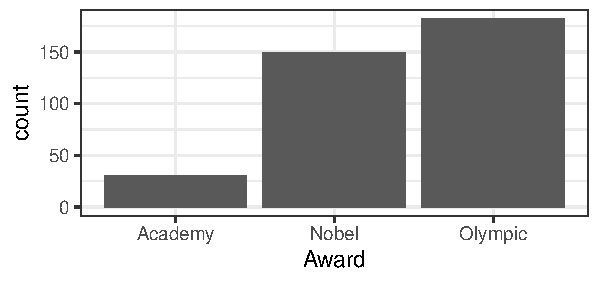
\includegraphics[width=.25\textwidth,height=.125\textwidth]{figure/unnamed-chunk-15-1} 

}


\end{knitrout}
\columnbreak

\begin{knitrout}\small
\definecolor{shadecolor}{rgb}{0.969, 0.969, 0.969}\color{fgcolor}\begin{kframe}
\begin{alltt}
\hlkwd{gf_props}\hldef{(}\hlopt{~}\hldef{Award,}\hlkwc{data}\hldef{=StudentSurvey,}
         \hlkwc{fill} \hldef{=} \hlsng{"forestgreen"}\hldef{)}
\end{alltt}
\end{kframe}

{\centering 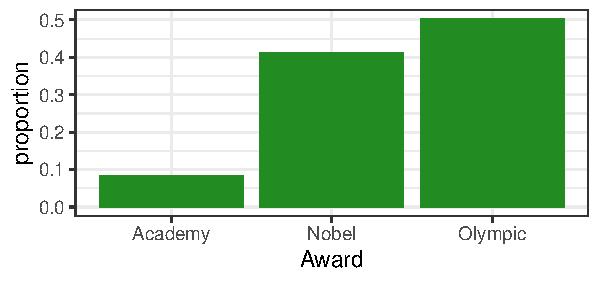
\includegraphics[width=.25\textwidth,height=.125\textwidth]{figure/unnamed-chunk-16-1} 

}


\end{knitrout}

\vspace*{-.15in}
\subsection*{Two Categorical}


\begin{knitrout}\small
\definecolor{shadecolor}{rgb}{0.969, 0.969, 0.969}\color{fgcolor}\begin{kframe}
\begin{alltt}
\hlkwd{tally}\hldef{(}\hlopt{~} \hldef{Award} \hlopt{+} \hldef{Smoke ,} \hlkwc{data} \hldef{= StudentSurvey)}
\end{alltt}
\begin{verbatim}
         Smoke
Award      No Yes
  Academy  29   2
  Nobel   129  20
  Olympic 161  21
\end{verbatim}
\end{kframe}
\end{knitrout}
\vspace*{-.20in}
\begin{knitrout}\small
\definecolor{shadecolor}{rgb}{0.969, 0.969, 0.969}\color{fgcolor}\begin{kframe}
\begin{alltt}
\hlkwd{tally}\hldef{(}\hlopt{~} \hldef{Award} \hlopt{+} \hldef{Smoke ,} \hlkwc{format} \hldef{=} \hlsng{"proportion"}\hldef{,}
      \hlkwc{data} \hldef{= StudentSurvey)}
\end{alltt}
\begin{verbatim}
         Smoke
Award           No      Yes
  Academy 0.080110 0.005525
  Nobel   0.356354 0.055249
  Olympic 0.444751 0.058011
\end{verbatim}
\end{kframe}
\end{knitrout}
\vspace*{-.20in}
\begin{knitrout}\small
\definecolor{shadecolor}{rgb}{0.969, 0.969, 0.969}\color{fgcolor}\begin{kframe}
\begin{alltt}
\hlkwd{tally}\hldef{(}\hlopt{~} \hldef{Award} \hlopt{+} \hldef{Smoke ,} \hlkwc{format} \hldef{=} \hlsng{"percent"}\hldef{,}
      \hlkwc{margins} \hldef{=} \hlnum{TRUE}\hldef{,} \hlkwc{data} \hldef{= StudentSurvey)}
\end{alltt}
\begin{verbatim}
         Smoke
Award           No      Yes    Total
  Academy   8.0110   0.5525   8.5635
  Nobel    35.6354   5.5249  41.1602
  Olympic  44.4751   5.8011  50.2762
  Total    88.1215  11.8785 100.0000
\end{verbatim}
\end{kframe}
\end{knitrout}
\vspace*{-.20in}

\begin{knitrout}\small
\definecolor{shadecolor}{rgb}{0.969, 0.969, 0.969}\color{fgcolor}\begin{kframe}
\begin{alltt}
\hlkwd{tally}\hldef{(}\hlopt{~} \hldef{Award} \hlopt{|} \hldef{Smoke ,} \hlkwc{data}\hldef{=StudentSurvey,}
      \hlkwc{format} \hldef{=} \hlsng{"proportion"}\hldef{)}
\end{alltt}
\begin{verbatim}
         Smoke
Award          No     Yes
  Academy 0.09091 0.04651
  Nobel   0.40439 0.46512
  Olympic 0.50470 0.48837
\end{verbatim}
\end{kframe}
\end{knitrout}
\vspace*{-.20in}
\begin{knitrout}\small
\definecolor{shadecolor}{rgb}{0.969, 0.969, 0.969}\color{fgcolor}\begin{kframe}
\begin{alltt}
\hlkwd{tally}\hldef{(}\hlopt{~} \hldef{Award} \hlopt{|} \hldef{Smoke ,} \hlkwc{data}\hldef{=StudentSurvey,}
      \hlkwc{format} \hldef{=} \hlsng{"percent"}\hldef{)}
\end{alltt}
\begin{verbatim}
         Smoke
Award         No    Yes
  Academy  9.091  4.651
  Nobel   40.439 46.512
  Olympic 50.470 48.837
\end{verbatim}
\end{kframe}
\end{knitrout}
\vspace*{-.20in}

\begin{knitrout}\small
\definecolor{shadecolor}{rgb}{0.969, 0.969, 0.969}\color{fgcolor}\begin{kframe}
\begin{alltt}
\hlkwd{tally}\hldef{(}\hlopt{~} \hldef{Award} \hlopt{|} \hldef{Smoke,} \hlkwc{data}\hldef{=StudentSurvey,}
      \hlkwc{format} \hldef{=} \hlsng{"proportion"}\hldef{,} \hlkwc{margins} \hldef{=} \hlnum{TRUE}\hldef{)}
\end{alltt}
\begin{verbatim}
         Smoke
Award          No     Yes
  Academy 0.09091 0.04651
  Nobel   0.40439 0.46512
  Olympic 0.50470 0.48837
  Total   1.00000 1.00000
\end{verbatim}
\end{kframe}
\end{knitrout}

\end{multicols}
\newpage
\chead{\sf \bfseries \Large R Sampler for Applied Statistics (cont'd)}
\begin{multicols}{3}


\begin{knitrout}\small
\definecolor{shadecolor}{rgb}{0.969, 0.969, 0.969}\color{fgcolor}\begin{kframe}
\begin{alltt}
\hlkwd{gf_bar}\hldef{(}\hlopt{~}\hldef{Sex,} \hlkwc{fill} \hldef{=} \hlopt{~}\hldef{Award,} \hlkwc{data}\hldef{=StudentSurvey)}
\end{alltt}
\end{kframe}

{\centering 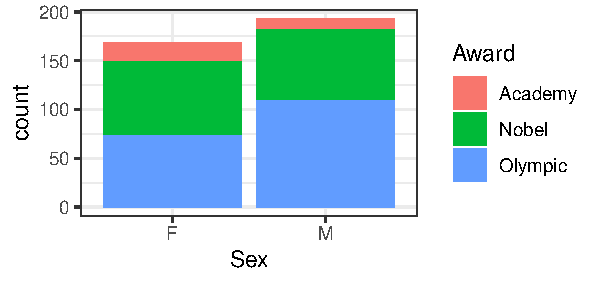
\includegraphics[width=.25\textwidth,height=.125\textwidth]{figure/unnamed-chunk-24-1} 

}


\end{knitrout}
\vspace*{-.20in}
\begin{knitrout}\small
\definecolor{shadecolor}{rgb}{0.969, 0.969, 0.969}\color{fgcolor}\begin{kframe}
\begin{alltt}
\hlkwd{gf_props}\hldef{(}\hlopt{~}\hldef{Sex,} \hlkwc{fill} \hldef{=} \hlopt{~}\hldef{Award,} \hlkwc{data}\hldef{=StudentSurvey)}
\end{alltt}
\end{kframe}

{\centering 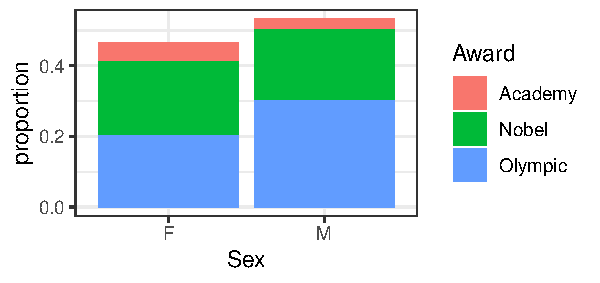
\includegraphics[width=.25\textwidth,height=.125\textwidth]{figure/unnamed-chunk-25-1} 

}


\end{knitrout}
\vspace*{-.20in}





\begin{knitrout}\small
\definecolor{shadecolor}{rgb}{0.969, 0.969, 0.969}\color{fgcolor}\begin{kframe}
\begin{alltt}
\hlkwd{gf_props}\hldef{(}\hlopt{~}\hldef{Sex,} \hlkwc{fill} \hldef{=} \hlopt{~}\hldef{Award,} \hlkwc{position} \hldef{=} \hlsng{"stack"}\hldef{,}
         \hlkwc{data}\hldef{=StudentSurvey)}
\end{alltt}
\end{kframe}

{\centering 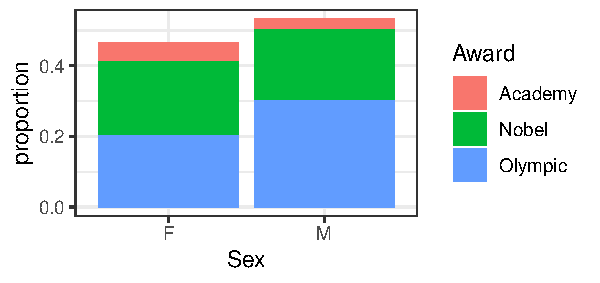
\includegraphics[width=.25\textwidth,height=.125\textwidth]{figure/unnamed-chunk-26-1} 

}


\end{knitrout}
\vspace*{-.20in}

\begin{knitrout}\small
\definecolor{shadecolor}{rgb}{0.969, 0.969, 0.969}\color{fgcolor}\begin{kframe}
\begin{alltt}
\hlkwd{gf_props}\hldef{(}\hlopt{~}\hldef{Sex,} \hlkwc{fill} \hldef{=} \hlopt{~}\hldef{Award,}
         \hlkwc{position} \hldef{=} \hlsng{"dodge"}\hldef{,} \hlkwc{data}\hldef{=StudentSurvey)}
\end{alltt}
\end{kframe}

{\centering 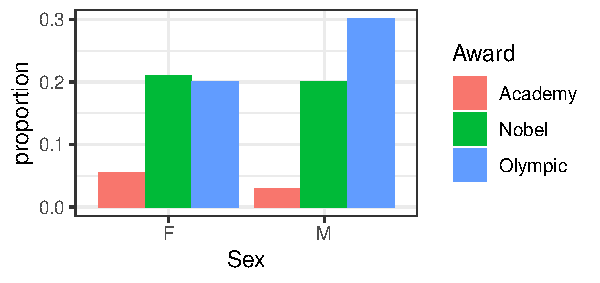
\includegraphics[width=.25\textwidth,height=.125\textwidth]{figure/unnamed-chunk-27-1} 

}


\end{knitrout}
%\vspace*{-.20in}
\columnbreak
\begin{knitrout}\small
\definecolor{shadecolor}{rgb}{0.969, 0.969, 0.969}\color{fgcolor}\begin{kframe}
\begin{alltt}
\hlkwd{gf_props}\hldef{(}\hlopt{~}\hldef{Sex,} \hlkwc{fill} \hldef{=} \hlopt{~}\hldef{Award,}
         \hlkwc{position} \hldef{=} \hlsng{"fill"}\hldef{,} \hlkwc{data}\hldef{=StudentSurvey)}
\end{alltt}
\end{kframe}

{\centering 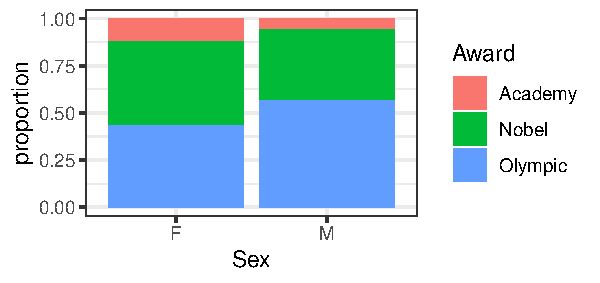
\includegraphics[width=.25\textwidth,height=.125\textwidth]{figure/unnamed-chunk-28-1} 

}


\end{knitrout}
\vspace*{-.20in}

\subsection*{One Quantitative}
%\columnbreak
\begin{knitrout}\small
\definecolor{shadecolor}{rgb}{0.969, 0.969, 0.969}\color{fgcolor}\begin{kframe}
\begin{alltt}
\hlkwd{gf_histogram}\hldef{(}\hlopt{~} \hldef{Height,} \hlkwc{data} \hldef{= StudentSurvey)}
\end{alltt}
\end{kframe}

{\centering 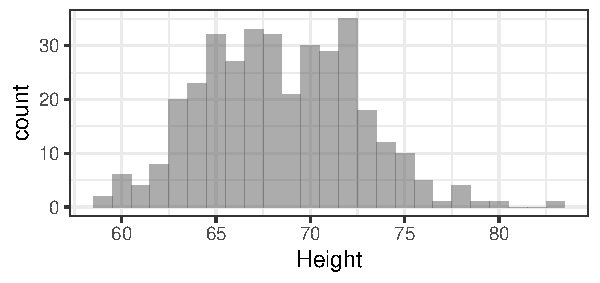
\includegraphics[width=.25\textwidth,height=.125\textwidth]{figure/stu-hist1-1} 

}


\end{knitrout}
\vspace*{-.20in}
\begin{knitrout}\small
\definecolor{shadecolor}{rgb}{0.969, 0.969, 0.969}\color{fgcolor}\begin{kframe}
\begin{alltt}
\hlkwd{gf_histogram}\hldef{(}\hlopt{~} \hldef{Height} \hlopt{|} \hldef{Sex} \hlopt{~} \hldef{.,}
             \hlkwc{data} \hldef{= StudentSurvey,} \hlkwc{binwidth} \hldef{=} \hlnum{2}\hldef{)}
\end{alltt}
\end{kframe}

{\centering 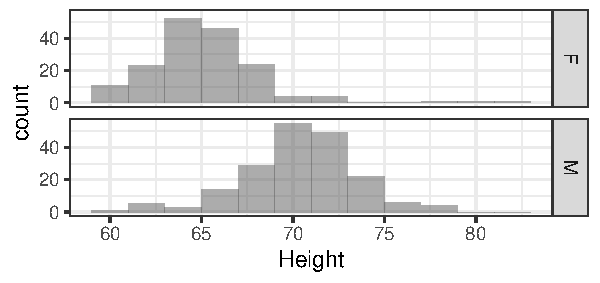
\includegraphics[width=.25\textwidth,height=.125\textwidth]{figure/stu-hist2-1} 

}


\end{knitrout}
%\columnbreak

\subsection*{One Quantitative and One Categorical}
\vspace*{-.15in}

\begin{knitrout}\small
\definecolor{shadecolor}{rgb}{0.969, 0.969, 0.969}\color{fgcolor}\begin{kframe}
\begin{alltt}
\hlkwd{favstats}\hldef{(TV} \hlopt{~} \hldef{Sex,} \hlkwc{data} \hldef{= StudentSurvey)}
\end{alltt}
\begin{verbatim}
  Sex min Q1 median Q3 max  mean    sd
1   F   0  3      4  6  20 5.237 4.100
2   M   0  3      5 10  40 7.620 6.427
    n missing
1 169       0
2 192       1
\end{verbatim}
\end{kframe}
\end{knitrout}
\vspace*{-.15in}

\begin{knitrout}\small
\definecolor{shadecolor}{rgb}{0.969, 0.969, 0.969}\color{fgcolor}\begin{kframe}
\begin{alltt}
\hlkwd{gf_boxplot}\hldef{(TV} \hlopt{~} \hldef{Sex,} \hlkwc{data} \hldef{= StudentSurvey)}
\end{alltt}
\end{kframe}

{\centering 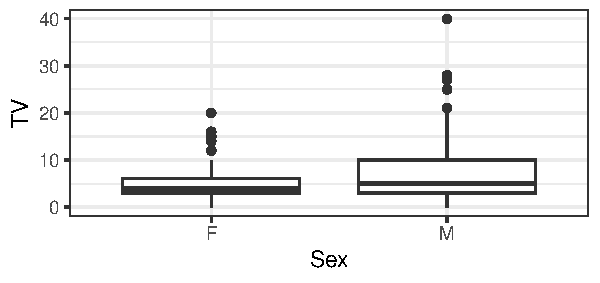
\includegraphics[width=.25\textwidth,height=.125\textwidth]{figure/bwplot-1} 

}


\end{knitrout}
\vspace*{-.15in}

\subsection*{Two Quantitative}
\vspace*{-.15in}

%\columnbreak
%\iffalse
\begin{knitrout}\small
\definecolor{shadecolor}{rgb}{0.969, 0.969, 0.969}\color{fgcolor}\begin{kframe}
\begin{alltt}
\hlkwd{gf_point}\hldef{(Weight} \hlopt{~} \hldef{Height,} \hlkwc{data} \hldef{= StudentSurvey)}
\end{alltt}
\end{kframe}

{\centering 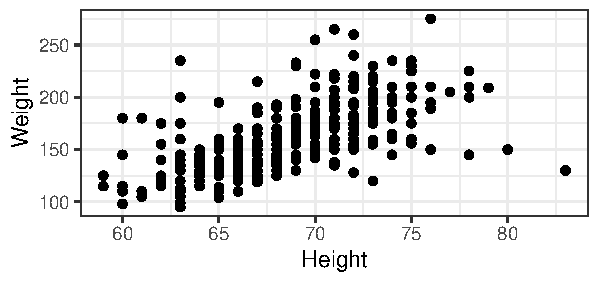
\includegraphics[width=.25\textwidth,height=.125\textwidth]{figure/unnamed-chunk-29-1} 

}


\end{knitrout}
\vspace*{-.20in}
\begin{knitrout}\footnotesize
\definecolor{shadecolor}{rgb}{0.969, 0.969, 0.969}\color{fgcolor}\begin{kframe}
\begin{alltt}
\hlkwd{gf_point}\hldef{(Weight} \hlopt{~} \hldef{Height,} \hlkwc{data} \hldef{= StudentSurvey)  |>}
  \hlkwd{gf_smooth}\hldef{()}
\end{alltt}
\end{kframe}

{\centering 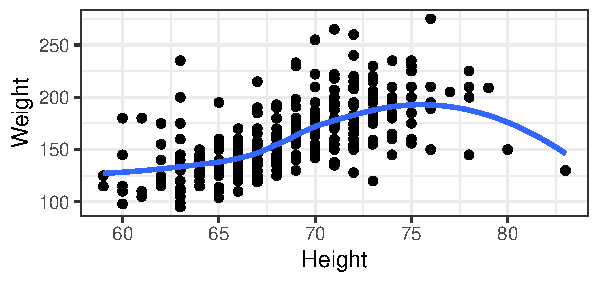
\includegraphics[width=.25\textwidth,height=.125\textwidth]{figure/unnamed-chunk-30-1} 

}


\end{knitrout}
\vspace*{-.20in}
\begin{knitrout}\footnotesize
\definecolor{shadecolor}{rgb}{0.969, 0.969, 0.969}\color{fgcolor}\begin{kframe}
\begin{alltt}
\hlkwd{gf_point}\hldef{(Weight} \hlopt{~} \hldef{Height,} \hlkwc{data} \hldef{= StudentSurvey)  |>}
  \hlkwd{gf_smooth}\hldef{(}\hlkwc{method} \hldef{=} \hlsng{"lm"}\hldef{)}
\end{alltt}
\end{kframe}

{\centering 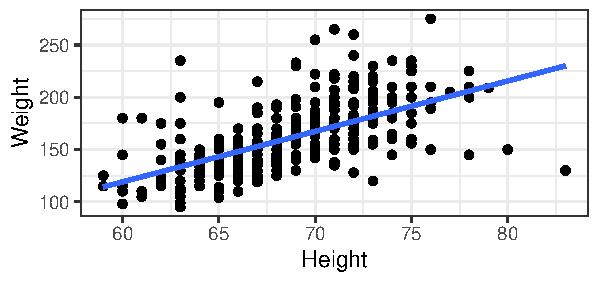
\includegraphics[width=.25\textwidth,height=.125\textwidth]{figure/unnamed-chunk-31-1} 

}


\end{knitrout}
\vspace*{-.20in}
\end{multicols}

\newpage
\chead{\sf \bfseries \Large R Sampler for Applied Statistics (cont'd)}
\begin{multicols}{2}


\begin{knitrout}\small
\definecolor{shadecolor}{rgb}{0.969, 0.969, 0.969}\color{fgcolor}\begin{kframe}
\begin{alltt}
\hlkwd{gf_point}\hldef{(Weight} \hlopt{~} \hldef{Height,} \hlkwc{color} \hldef{=} \hlopt{~} \hldef{Sex,} \hlkwc{data} \hldef{= StudentSurvey)}
\end{alltt}
\end{kframe}

{\centering 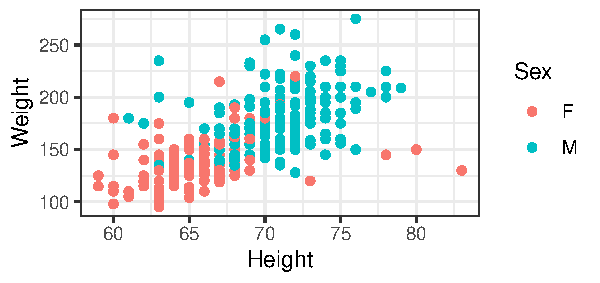
\includegraphics[width=.25\textwidth,height=.125\textwidth]{figure/unnamed-chunk-33-1} 

}


\end{knitrout}
\vspace*{-.20in}
\begin{knitrout}\footnotesize
\definecolor{shadecolor}{rgb}{0.969, 0.969, 0.969}\color{fgcolor}\begin{kframe}
\begin{alltt}
\hlkwd{gf_point}\hldef{(Weight} \hlopt{~} \hldef{Height,} \hlkwc{color} \hldef{=} \hlopt{~} \hldef{Sex,} \hlkwc{data} \hldef{= StudentSurvey)  |>}
  \hlkwd{gf_smooth}\hldef{()}
\end{alltt}
\end{kframe}

{\centering 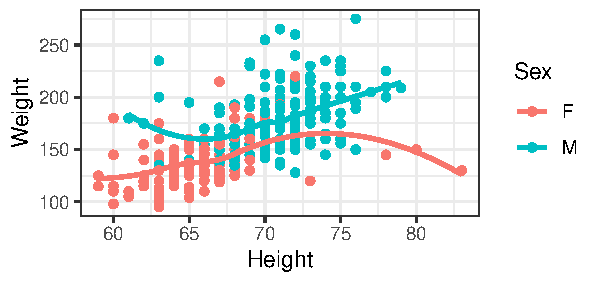
\includegraphics[width=.25\textwidth,height=.125\textwidth]{figure/unnamed-chunk-34-1} 

}


\end{knitrout}
%\fi

%\iffalse
\begin{knitrout}\small
\definecolor{shadecolor}{rgb}{0.969, 0.969, 0.969}\color{fgcolor}\begin{kframe}
\begin{alltt}
\hldef{model} \hlkwb{<-} \hlkwd{lm}\hldef{(Weight} \hlopt{~} \hldef{Height,} \hlkwc{data} \hldef{= StudentSurvey)}
\hlkwd{summary}\hldef{(model)}
\end{alltt}
\begin{verbatim}

Call:
lm(formula = Weight ~ Height, data = StudentSurvey)

Residuals:
    Min      1Q  Median      3Q     Max 
-100.05  -13.81   -3.06   11.76  101.41 

Coefficients:
            Estimate Std. Error t value
(Intercept) -170.269     22.412    -7.6
Height         4.823      0.327    14.8
            Pr(>|t|)
(Intercept)  2.8e-13
Height       < 2e-16

Residual standard error: 24.9 on 350 degrees of freedom
  (10 observations deleted due to missingness)
Multiple R-squared:  0.384,	Adjusted R-squared:  0.382 
F-statistic:  218 on 1 and 350 DF,  p-value: <2e-16
\end{verbatim}
\end{kframe}
\end{knitrout}
%\fi


%\vfill
\end{multicols}




\end{document}



